\section{Implementation}
\label{sec:implementation}

\begin{figure}[t]
    \centering
    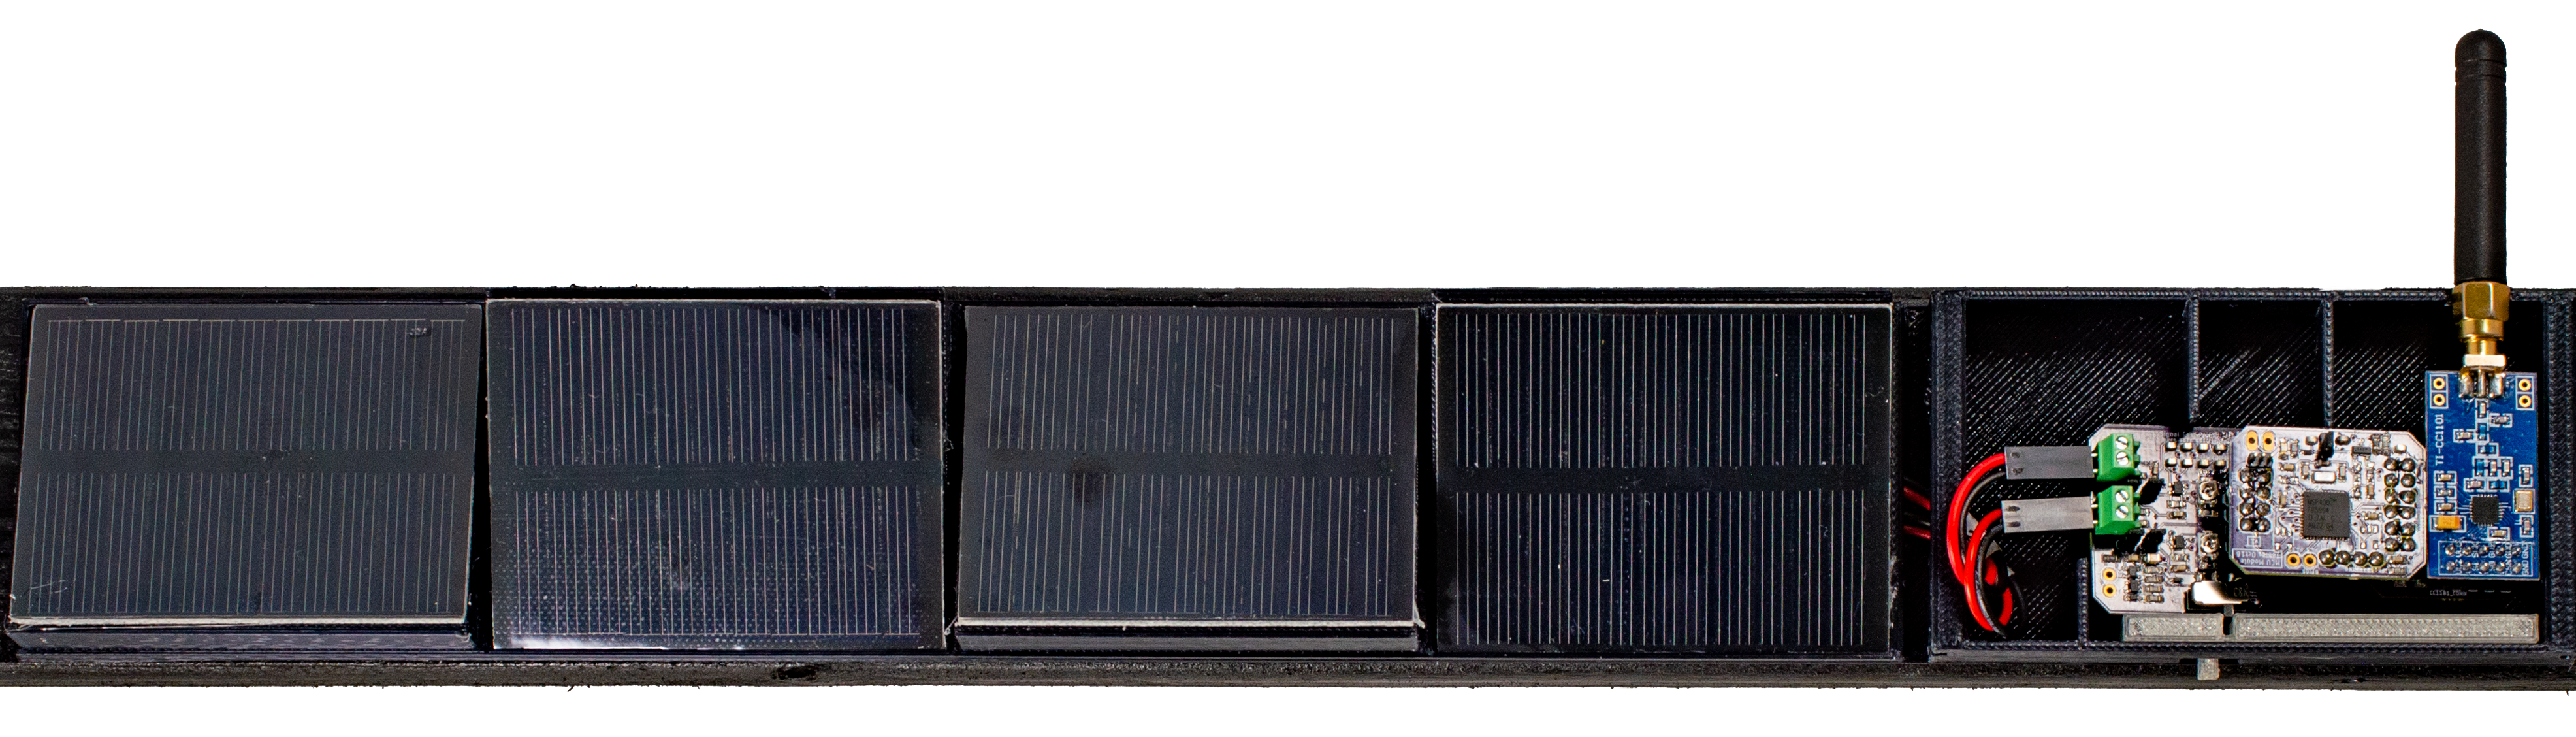
\includegraphics[width=\columnwidth]{figs/full_waldo_open_cropped.png}
    \caption{3D printed solar panel and PCB housing enclosure with angled slots for solar energy harvesters and the \sysname prototype PCB.}
    \label{fig:mounting}
\end{figure}    

%\begin{figure*}[t]
%    \centering
%    \begin{subfigure}[b]{0.5\textwidth}
%        \centering
%        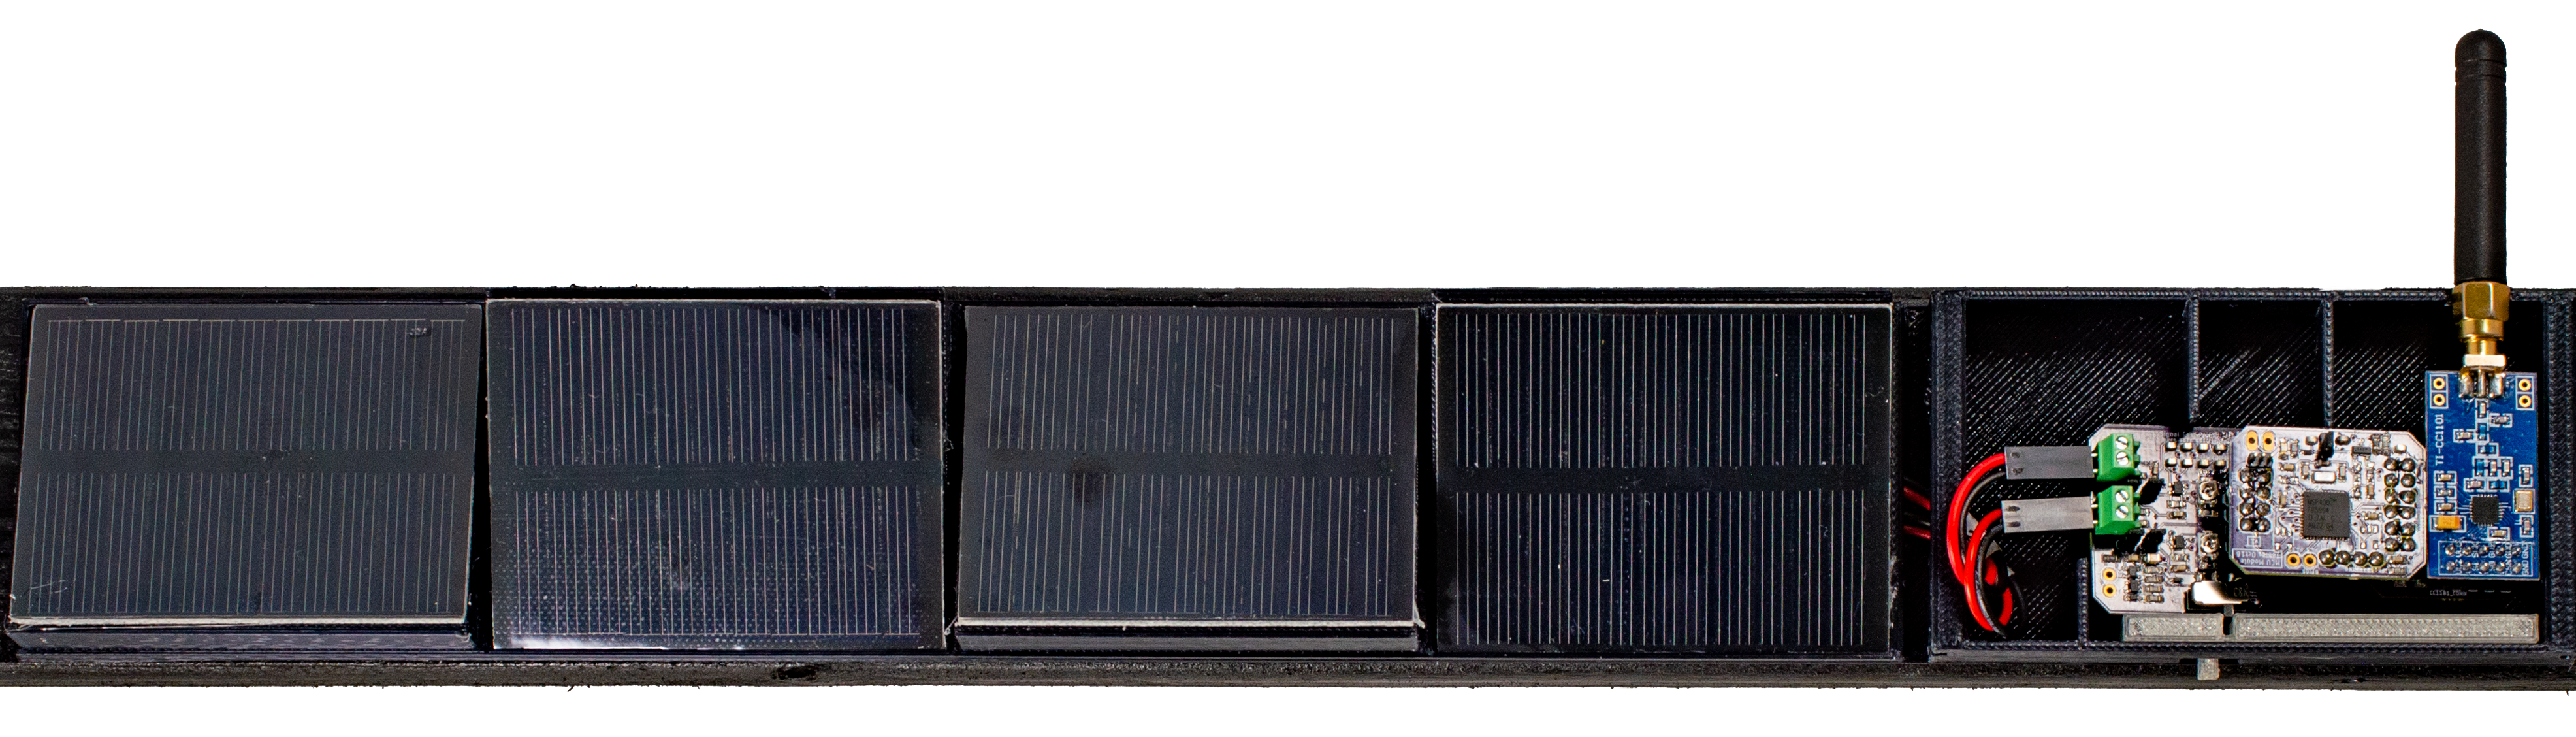
\includegraphics[width=\columnwidth]{figs/full_waldo_open_cropped.png}
%        \caption{3D printed solar panel enclosure with angled slots for solar energy harvesters.}
%        \label{fig:mounting}
%    \end{subfigure}%
    %
%    \begin{subfigure}[b]{0.5\textwidth}
%        \centering
%        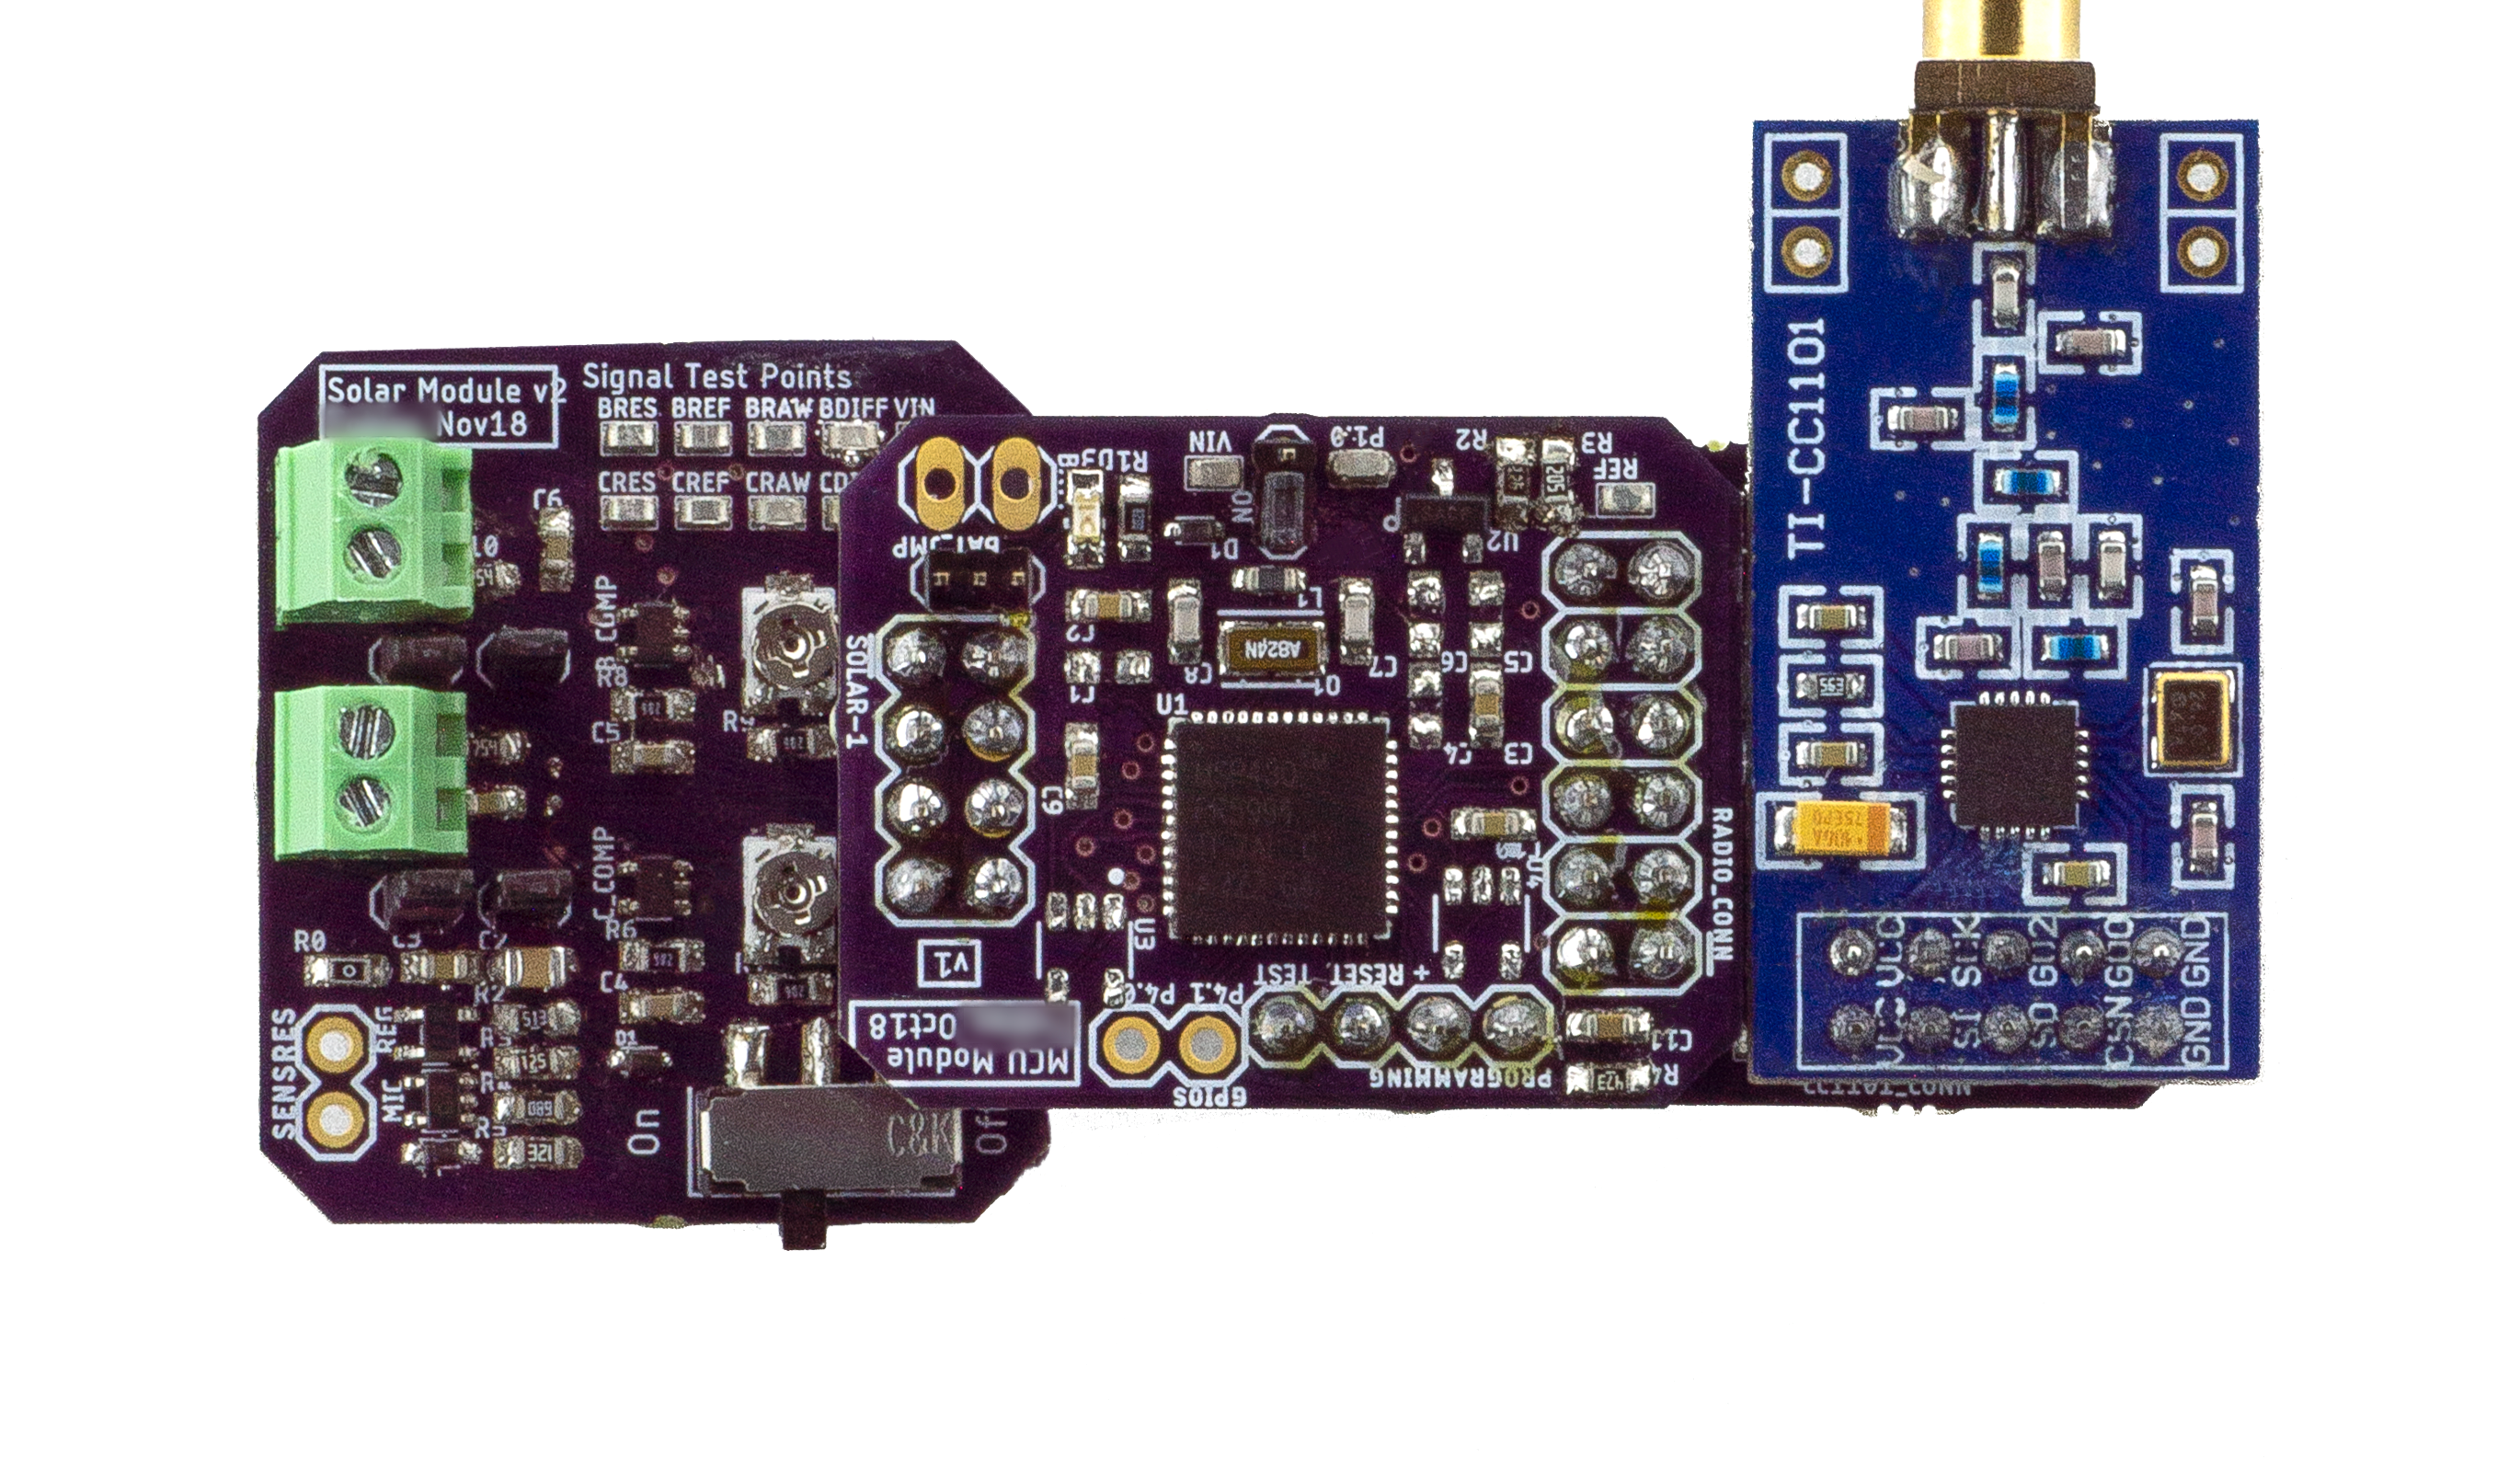
\includegraphics[width=0.75\columnwidth]{figs/waldoguts-anon-white.png}
%        \caption{ \sysname prototype PCB.}
%        \label{fig:pcb}
%    \end{subfigure}
%    \caption{\sysname implementation \label{fig:prototype}}
%\end{figure*}

In order to evaluate our approach, we implemented a prototype \sysname sensor that includes custom hardware (shown in \figref{fig:mounting}), firmware for detecting and reporting doorway events, and a custom 3D~printed doorway mounting system that holds the assembled PCB and solar panels in a slim profile~(\figref{fig:mounting}).

\noindpar{Hardware:} Our prototype hardware integrates four~(4)~RL-55x70 solar panels~(70.00mm x 55.00mm) and custom printed circuit boards~(PCB) housed in a 3D-printed plastic enclosure.
The prototype uses an MSP430FR5994 microcontroller from Texas Instrument's~(TI) FRAM line of ultra-low-power processors.
The newest FRAM-based MSP430s have several advantages over previous models: lower sleep-mode currents, shorter wake-up latencies, and faster non-volatile FRAM.
Entirely interrupt-driven and remaining asleep most of the time to conserve energy, \sysname benefits from these improvements.
The solar panels are connected in two angled series-connected banks, each consisting of two series-connected panels.
We connect the panels in series to increase voltage to allow \sysname to work in a wider range of lighting conditions and make doorway events easier to detect.
Our panels---chosen to provide flexibility during prototyping---provide enough current to power the circuit with sufficient voltage levels for detection under a wide range of lighting conditions.
Future designs will focus on miniaturization.
The detector circuitry is made using nano-power comparators (TI~TLV3691) and a passive RC filter network. In order to give us flexibility, the RC filter network is tunable using trim potentiometers pre-installation or digital potentiometers in deployment.  
The \sysname PCB also has a TI~CC1101 radio for communication.
The hardware used in the \sysname prototype, shown in \figref{fig:mounting}, is not prohibitively expensive or obtrusive.

\begin{table}[t]
\centering
\footnotesize
\begin{tabular}{@{}p{1.4in}llc@{}}
\toprule
\textbf{Components}          & \multicolumn{1}{r}{\textbf{Cost per unit}} & \multicolumn{1}{r}{\textbf{Unit Cost for 1000}} \\ \midrule
\textit{Solar Panels}       	& \$ 1.95	&  \$ 1.76	 \\
\textit{Microcontroller (MSP430FR5994)} & \$ 8.04 & \$ 5.09	\\
\textit{Wireless~RF~Transceiver (CC1101)} & \$ 9.40	 & \$ 9.40	\\
\textit{Components} & \$ 17.02	& \$ 6.63     \\ 
\textit{PCBs*} & \$ 2.94	& \$ 0.30     \\ \midrule
\textit{Entire \sysname Prototype} & \$ 39.35	& \$ 23.18    \\ \midrule
\end{tabular}
\caption{Breakdown of the \sysname prototype costs at time of purchase for development.}
\label{tab:costbreakdown}
\end{table}

The total cost of the current prototype at the time of purchase, including all PCBs, component parts, Radio modules, and solar panels is \$23.18 per unit if ordered in quantities of 1000\footnote{PCBs priced by \url{seeedstudio.com}.}.
The distribution of the prototype costs is shown in Table~\ref{tab:costbreakdown}.
The current prototype has several components that are meant to enable experimentation and testing (modular board design, jumpers, headers, test points, etc)---a commercial version of \sysname will be dramatically cheaper and smaller.



\noindpar{Firmware:} %This is now up2date -NT 4/1
The \sysname firmware implements the detection algorithm with a trained decision tree for event classification discussed in \secref{sec:system}.
Monitoring the interrupts from the detectors and deducing the direction of motion upon triggering are the main tasks of the system.
The firmware is designed to be ultra-low power, even in active mode, and has low computational complexity, offloading the bulk of the detection to the hardware circuits.
The \sysname firmware is composed of 691~lines of commented C code, compiling to a 4459~byte image. This code size comprises only 1.7\% of the available code space on the MSP430FR5994~(256KB), leaving ample room for implementing custom tasks, recognizers, or multiprogramming operating systems.

\noindpar{Mechanical Design:} %Dimensions are current-NT 4/1
The 3D printed mounting system (shown in \figref{fig:mounting}) is made of PLA plastic and contains the PCB, solar cells, and necessary wiring connecting them.
\sysname's 3D printed enclosure measures \SI{56.0}{\milli\meter} by \SI{395.9}{\milli\meter} by \SI{22.8}{\milli\meter} at its thickest point. The enclosure provides a nesting place for the solar cells, pointing downward. 
A simple slide-mounted cap was also designed to cover the PCB housing to help minimize distractions when deployed.  The sensor could be minimized further by selecting smaller solar panels and by placing the PCB behind the panels rather than to the side of the panels.
The angle of the solar cell slots is set such that half of the solar cells tend toward the entry, while the rest face toward the exit.

All software, firmware, hardware schematics and layouts, and 3D printed mounting system will be made freely available at publication time.
